
\section{La Web Semántica}

En 1989 Tim Berners-Lee realizó para el CERN un modelo de gestión de la 
información basado en un sistema distribuido de hipertexto\footnote{\url{http://www.w3.org/Proposal}}. 
Fue el origen de lenguaje de marcado HTML y la semilla de la Web actual.

Era evidente que resultaría muy difícil encontrarla y usarla eficientemente. 
Así el propio Tim Berners-Lee 
expondría\footnote{\url{http://www.scientificamerican.com/article.cfm?articleID=00048144-10D2-1C70-84A9809EC588EF21&catID=2}}
en 2001 su visión\footnote{Cita extraída de las transparencias de José Emilio 
Labra Gayo para el curso de verano sobre Web Semántica de la Universidad de 
Oviedo, \url{http://www.di.uniovi.es/~labra/cursos/ver06/}} de la Web Semántica:

\begin{quote}
	\emph{«... \textbf{disponer datos} en la Web \textbf{definidos y enlazados} 
	de forma que puedan ser \textbf{utilizados por las máquinas}, no solamente 
	para visualizarnos, sino también para \textbf{automatizar} tareas, 
	\textbf{integrar} y \textbf{reutilizar} datos entre aplicaciones.»}
\end{quote} 

Y quizás se está dedicando mucho esfuerzo a publicar y procesar de forma autónoma
esos datos, obviando quizás la parte más importante: 
\textbf{enlazarlos}\footnote{Traducción libre de un extracto de un documento (\url{http://www.w3.org/DesignIssues/LinkedData}) de Tim Berners-Lee}.

\begin{quote}
	\emph{«La Web Semántica no sólo se trata de publicar datos en la Web. Se 
	trata de enlazarlos para que personas o máquinas podamos explorar esos 
	datos. Al estar enlazados, podremos encontrar fácilmente datos relacionados 
	con los datos que disponemos.»}
\end{quote}

\subsection{Evolución de la Web}

La Web es un recurso muy especial y particular, con unas características muy 
especiales que deben tenerse en cuenta: no centralizada, información dinámica,
mucha cantidad de información y está abierta a todo el mundo.

\begin{figure}[H]
	\centering
	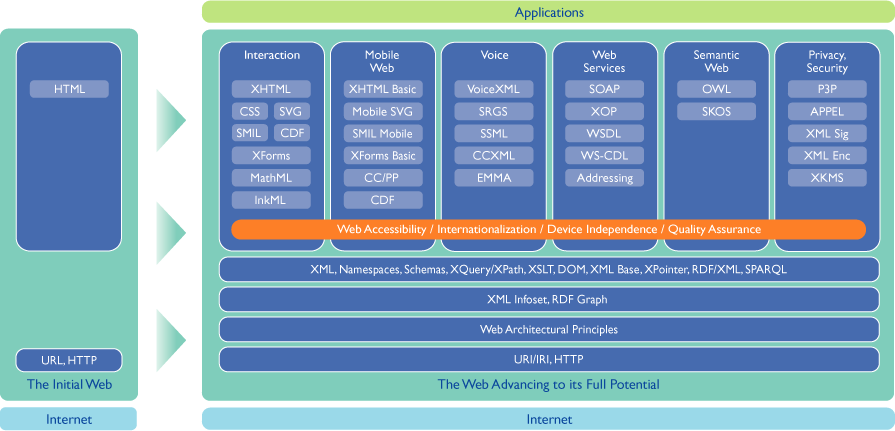
\includegraphics[width=12cm]{images/web-evolution.png}
	\caption{Evolución de la Web}
	\label{fig:evoWeb}
\end{figure}

En los últimos años la Web ha experimentado una notable evolución, como puede 
verse en la figura \ref{fig:evoWeb}\footnote{Fuente: W3C}, que le ha llevado a 
convertirse no sólo en un almacén de contenido estático, sino también en un 
repositorio universal de conocimiento y servicios.

A pesar de todas estas pequeñas revoluciones, todavía seguimos en una web 
\emph{sintáctica}. Hoy en día la llamada \emph{Web 2.0}\cite{O'Reilly2005} está
de actualidad, aunque todavía es una Web en la es muy difícil realizar muchas 
tareas que con la Web Semántica (\emph{¿Web 3.0?}), y todas sus tecnologías, 
al menos serán un poco más fácil de hacer.

\subsection{Estructura de la Web Semántica}

La Web Semántica se encuentra estructurada en capas (la llamada \emph{tarta de 
la Web Semántica}), de forma que se pudiera trabajar en cada uno de estos
sustratos de manera independiente a el estado de la implementación de las
capas inferiores y/o superiores.

Algunas parte del diseño aún se están discutiendo en los distintos grupos de
trabajo, aunque en la figura \ref{fig:swStack} encontramos el diseño que toma
más forma después de los últimos años de trabajo:

\begin{figure}[H]
	\centering
	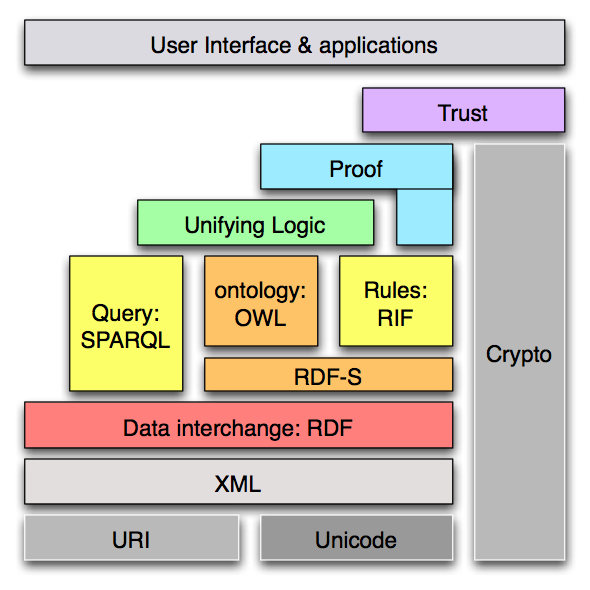
\includegraphics[width=10cm]{images/semantic-web-stack.png}
	\caption{Pila de la web semántica}
	\label{fig:swStack}
\end{figure}

Puede verse que el núcleo de la Web Semántica se construye sobre tres 
tecnologías fundamentales:

\begin{itemize}
  \item RDF\cite{Graham2004}
  \item OWL\cite{OWL}
  \item SPARQL\cite{Eric2006}
\end{itemize}

Con una envoltura de lógica y reglas, sustentadas sobre una infraestructura 
basada en XML, URI's y Unicode.

Véase que las reglas están a mismo nivel que las ontologías, y no por
encima como se pensaba en los primeros diseños, por la íntima relación que ambas
tienen.

\subsection{Elementos}

\subsubsection{Elementos básicos}

\paragraph{Unicode}es una iniciativa\footnote{\url{http://www.unicode.org/}} de 
un consorcio de empresas dedicadas a la internacionalización para conseguir una 
representación informática de los caracteres en todos los idiomas de forma que 
pueda ser representados y manipulados de forma universal. 

Aunque existen varias codificaciones distintas, UTF-8\cite{Yergeau2003} es la 
codificación unicode más usada y extendida, tanto por su sencillez (usa grupos 
de bytes) como por su flexibilidad (los alfabetos de muchos de los lenguajes 
del mundo se pueden representar en UTF-8).

Unicode es el recurso primario de representación de caracteres en la Web Semántica.

\paragraph{URI}acrónimo del inglés \emph{Uniform Resource Identifier}\cite{Berners-Lee1998}, 
identificador uniforme de recursos, es un mecanismo para la identificación de recursos
en red. Se trata de una especialización del IRI (Internationalized Resource Identifier) 
limitada al rango de caracteres ASCII.

Un concepto que mezcla URL\footnote{Uniform Resource Locator, localizador uniforme de recurso} 
y URN\footnote{Uniform Resource Name, nombre uniforme de recurso} para cumplir una doble 
funcionalidad: servir como protocolo de acceso e identificar de manera única los recursos 
en la World Wide Web.

\subsubsection{XML}

XML\cite{Bray2006} (eXtensible Markup Language\footnote{\url{http://www.w3.org/XML/}}, 
lenguaje  de marcado extensible) es un formato de marcado estructurado para la 
representación de información muy usado y extendido hoy en día, hasta tal punto de 
ser considerado el lenguaje universal para el intercambio de información. 

Desarrollado por el W3C a partir de SGML\footnote{\url{http://www.w3.org/MarkUp/SGML/}} 
con el objetivo que fuera fácilmente procesable por una máquina y legible por un 
humano. 

\begin{figure}[H]
\lstset{language=PeliculasXML}
\begin{lstlisting}
<?xml version="1.0" encoding="UTF-8"?>

<peliculas>

  <pelicula vista="true">
    <titulo>Resevoir Dogs</titulo>
    <autor>Quentin Tarantino</autor>
    <url>http://www.imdb.com/title/tt0105236/</url>
  </pelicula>

  <pelicula vista="false">
    ...
  </pelicula>

</peliculas>
\end{lstlisting}
\caption{Ejemplo de fichero en XML}
\label{fig:ejemplo.xml}
\end{figure}

Basándose en una definición abstracta (XML Schema\footnote{\url{http://www.w3.org/XML/Schema}}), 
permite extender su gramática de una forma muy fácil y sencilla de procesar 
(XSL/XSLT, XPath, XPointer, etc).

Es usado en múltiples tecnologías hoy en día, sobre todo en la web (XHTML, XForms, 
SVG, etc), aunque también para documentación (DocBook), interfaces de usuario (XUL,
Glade, XAML, etc), protocolos (Jabber), etc. Se utilizan espacios de nombres (namespace), 
identificados por URI's, para mezclar en un documento etiquetas pertenecientes a 
diferentes vocabularios.

Pero XML, a pesar de ser un lenguaje estructurado que es muy fácil de procesar, 
aún carece de la semántica necesaria. 

Sobre XML existe mucha bibliografía relacionada, siendo recomendable empezar por
\emph{XML Imprescindible}\cite{XMLNutshell}, un excelente libro que hace un amplio
recorrido por XML y todas sus tecnologías.

\subsubsection{RDF}

Acrónimo del inglés \emph{Resource Description Framework} (marco de descripción 
de recursos), RDF\footnote{\url{http://www.w3.org/RDF/}} es una especificación del 
W3C originalmente diseñada como modelo de metadatos, pero su uso se ha extendido como
método general para modelar el conocimiento.

RDF se basa en un modelo de tripletas del tipo \texttt{(sujeto, predicado, objeto)}. El
sujeto es un recurso que se identifica con una URI, y se relaciona mediante un 
predicado binario con el objeto, que puede ser otra URI o un literal.

\begin{figure}[H]
	\centering
	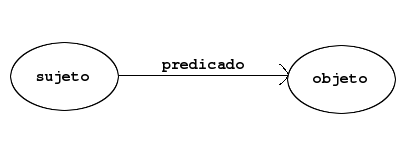
\includegraphics[width=10cm]{images/arc.png}
	\caption{Arco RDF}
	\label{fig:rdfTriplet}
\end{figure}

Cada tripleta puede verse como un arco, y al juntarse con otros arcos se obtiene
un grafo dirigido que describe los recursos y las relaciones entre todos los 
recursos.

Un ejemplo sencillo: \textit{Sergio Fdez es el creador de http://www.wikier.org/}. 
Usando Dublin Core (sección \ref{sec:dc}) podría quedar la siguiente tripleta: 
\texttt{(http://www.wikier.org/, dc:creator, "Sergio Fdez")}. Dando lugar a un 
grafo del estilo del que se puede ver en la figura~\ref{fig:rdfTripletExample}.

\begin{figure}[H]
	\centering
	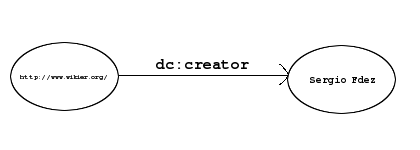
\includegraphics[width=12cm]{images/arc-example.png}
	\caption{Ejemplo de arco RDF}
	\label{fig:rdfTripletExample}
\end{figure}


RDF se puede serializar en tres sintaxis: 

\begin{itemize}
 \item XML\footnote{\url{http://www.w3.org/TR/rdf-syntax-grammar/}}
 \item N3\footnote{\url{http://www.w3.org/DesignIssues/Notation3}} (notación de tripletas)
 \item Turtle\footnote{\url{http://www.dajobe.org/2004/01/turtle/}}
\end{itemize}

El mismo grafo de la figura~\ref{fig:rdfTripletExample} se podría serializar 
con las tres sintaxis, conteniendo las tres representaciones idéntica información 
semántica:

\begin{figure}[H]
\lstset{language=RDF}
\begin{lstlisting}
<rdf:RDF xmlns:rdf="http://www.w3.org/1999/02/22-rdf-syntax-ns#"
         xmlns:rdfs="http://www.w3.org/2000/01/rdf-schema#"
         xmlns:dc="http://purl.org/dc/elements/1.1/"
>

  <rdf:Description rdf:about="http://www.wikier.org/">
    <dc:creator>Sergio Fdez</dc:creator>
  </rdf:Description>

</rdf:RDF>
\end{lstlisting}
\caption{Ejemplo de grafo RDF serializado en XML}
\label{fig:ejemplo.rdfxml}
\end{figure}

\begin{figure}[H]
\lstset{language=N3}
\begin{lstlisting}
@prefix dc <http://http://purl.org/dc/elements/1.1/>

<http://www.wikier.org> dc:creator "Sergio Fdez"
\end{lstlisting}
\caption{Ejemplo de grafo RDF serializado en N3}
\label{fig:ejemplo.rdfn3}
\end{figure}

\begin{figure}[H]
\lstset{language=Turtle}
\begin{lstlisting}
@prefix dc <http://http://purl.org/dc/elements/1.1/>

<http://www.wikier.org> 
	dc:creator "Sergio Fdez"
\end{lstlisting}
\caption{Ejemplo de grafo RDF serializado en Turtle}
\label{fig:ejemplo.rdfturtle}
\end{figure}

\subsubsection{RDFS}

RDFS (RDF Schema\cite{RDFS}) es una forma primitiva y limitada de describir 
ontologías en RDF, también llamado «\emph{vocabulario RDF}». Provee los elementos
básicos para la definición de ontologías (clases, subclases, propiedades, etc)
\footnote{¿Qué es una ontología? La mejor definición es la que da Tom Gruber
en \url{http://www-ksl.stanford.edu/kst/what-is-an-ontology.html}}.

Aunque OWL, del que hablaremos a continuación, es mucho más expresivo, aún muchas
ontologías se encuentras definidas con RDFS.

\subsubsection{OWL}

Acrónimo resultante de \emph{retorcer} el nombre de 
\emph{Web Ontology Language}, OWL\cite{OWL} es la recomendación 
oficial de W3C\footnote{\url{http://www.w3.org/}} para publicar ontologías en 
la Web. Se trata de un lenguaje de gran expresividad para describir conceptos 
y relaciones entre conceptos, con un compromiso entre expresividad y tratabilidad.

Es la versión revisada y mejorada de juntar dos lenguajes más viejos para la 
definición de ontologías como son DAML\footnote{\url{http://www.daml.org/}} y 
OIL\footnote{\url{http://www.ontoknowledge.org/oil/}} (lo llamado
DAML+OIL\footnote{\url{http://www.daml.org/2001/03/daml+oil-index}}).

La versión actual de OWL, la 1.0 (la 1.1 aún se encuentra en estos momentos en 
fase de desarrollo bajo el liderazgo del español Bernardo 
Cuenca\footnote{\url{http://www.cs.man.ac.uk/~bcg/}}), tiene 
tres variantes según su complejidad y expresividad:

\begin{itemize}
  \item \textbf{OWL Full}, íntimamente ligado a la lógica de RDF, pero que puede 
	resultar no computable.
  \item \textbf{OWL DL}, un subconjunto del anterior basado en la lógica 
	descriptiva ${SHOIN} (D)$.
  \item \textbf{OWL Lite}, subconjunto de OWL DL que se basa en la lógica 
	descriptiva de menor expresividad ${SHIF} (D)$.
\end{itemize}

Una perspectiva sencilla sería la mostrada por la figura~\ref{fig:owlVariants}.

\begin{figure}[H]
	\centering
	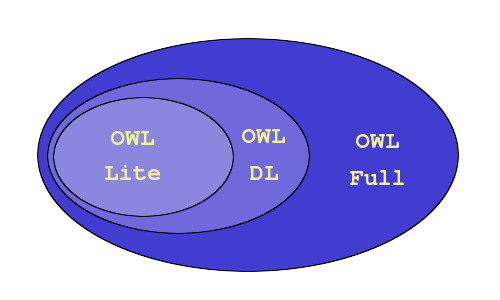
\includegraphics[width=12cm]{images/owl-variants.png}
	\caption{Perspectiva sencilla de OWL}
	\label{fig:owlVariants}
\end{figure}

Aunque el panorama no es tan sencillo, y para diferenciar cada una de ellas no
se puede hacer fijándose sólo en la complejidad, sino también en la parte de la 
lógica que abarcan. Quedando un panorama aún más confuso, como se puede ver en 
la figura \ref{fig:owlVariantsExtended}\footnote{Gráfico extraído de Ontotext, 
\url{http://www.ontotext.com/inference/rdfs_rules_owl.html#owl_fragments}}.

\begin{figure}[H]
	\centering
	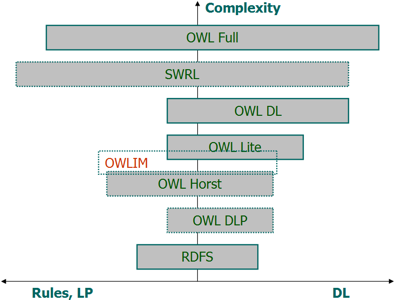
\includegraphics[width=10cm]{images/owl-dialects.png}
	\caption{Variantes de OWL ampliado}
	\label{fig:owlVariantsExtended}
\end{figure}

Hay que tener en cuenta que existe cierto solapamiento entre la expresividad de
OWL y la de RDFs (RDF-Schema), desvirtuando en cierta manera la visión original
por capas.

Para más información puede consultarse el último libro publicado acerca de 
OWL\cite{OWLBook}.

\subsubsection{SPARQL}

SPARQL\footnote{\url{http://www.w3.org/TR/rdf-sparql-query/}} es un nuevo lenguaje
de consulta sobre la base del conocimiento en OWL/RDF. No es el único\cite{ComparisonRDFQuery},
aunque si el más completo y la apuesta oficial del W3C en este área, debido a que es
un lenguaje con un compromiso en su justa medida entre semántica y 
complejidad\cite{SemanticsComplexitySPARQL}. 

Actualmente se trata del candidato a recomendación del W3C por parte del 
DAWG\footnote{\url{http://www.w3.org/2001/sw/DataAccess/}} (RDF Data Access Working 
Group).

Posee una sintaxis similar a la otros lenguajes de consulta relacionales, como
podría ser SQL. De hecho sus 
álgebras\footnote{\url{http://www.w3.org/2001/sw/DataAccess/rq23/rq24-algebra.html}} comparten\cite{RelationalAlgebraSPARQL} determinados puntos. 

\begin{figure}[H]
\lstset{language=SPARQL}
\begin{lstlisting}
PREFIX rdf: <http://www.w3.org/1999/02/22-rdf-syntax-ns#>
PREFIX dc: <http://purl.org/dc/elements/1.1/>

SELECT DISTINCT ?x, ?name
WHERE {
	?x dc:creator ?name
}
\end{lstlisting}
\caption{Ejemplo de consulta SPARQL}
\label{fig:ejemplo.sparql}
\end{figure}

Aplicando esta sencilla consulta de ejemplo a un RDF, como por ejemplo el de 
antes \ref{fig:ejemplo.rdfxml}, se obtendría el nombre del creador de cada recurso
definido.

A pesar de ser un lenguaje relativamente reciente, ya se encuentran disponibles
API's de consulta para numerosos lenguajes de programación: 
RDFLib\footnote{\url{http://rdflib.net/sparql/}} para Python, 
Jena\footnote{\url{http://jena.sourceforge.net/ARQ/}} en Java, 
Redland RDF\footnote{\url{http://librdf.org/}} en C con bindings también para 
otros lenguajes, twinql\footnote{\url{http://www.holygoat.co.uk/projects/twinql/}} 
en Lisp, etc. Además de estar soportado por alguno de los razonadores\footnote{Un 
razonador es un componente software que permite operar lógicamente sobre una base 
de conocimiento, por ejemplo para verificar su consistencia o inferir nueva
información.} más conocidos, como Pellet\footnote{\url{http://www.mindswap.org/2003/pellet/}} 
o KAON2\footnote{\url{http://kaon2.semanticweb.org/}}.

\subsection{Aplicaciones prácticas}

\subsubsection{Vocabularios RDF}

Existen multitud de vocabularios RDF para fines muy concretos, desde describir
personas, hasta eventos. Estos vocabularios suelen ser fácilmente extensibles y 
reutilizables entre si.

Existen multitud de ejemplos:

\begin{itemize}
  \item \textbf{Dublin Core\label{sec:dc}:} Dublin Core\footnote{\url{http://dublincore.org/}}, 
	también conocido por sus siglas \texttt{DC}, es un vocabulario RDF para la descripción 
	de múltiples propiedades de todo tipo de recursos online.

	Por ejemplo se ha usado Dublin Core en el ejemplo descrito en la 
	figura~\ref{fig:rdfTripletExample}, y evidentemente también en sus distintas 
	serializaciones (figura~\ref{fig:ejemplo.rdfxml}, figura~\ref{fig:ejemplo.rdfn3} 
	y figura~\ref{fig:ejemplo.rdfturtle}).

  \item \textbf{RSS:} Desarrollado en el seno de Netscape, RSS es el formato de sindicación de 
	noticias más extendido en la actualidad. Con un complicado historial, como se puede ver 
	en la figura~\ref{fig:rssEvolution}, de versiones incompatibles entre sí; de hecho sólo 
	la versión 1.0 de RSS es RDF, el resto de versiones han introducido ciertos aspectos
	incompatibles.

	\begin{figure}[H]
		\centering
		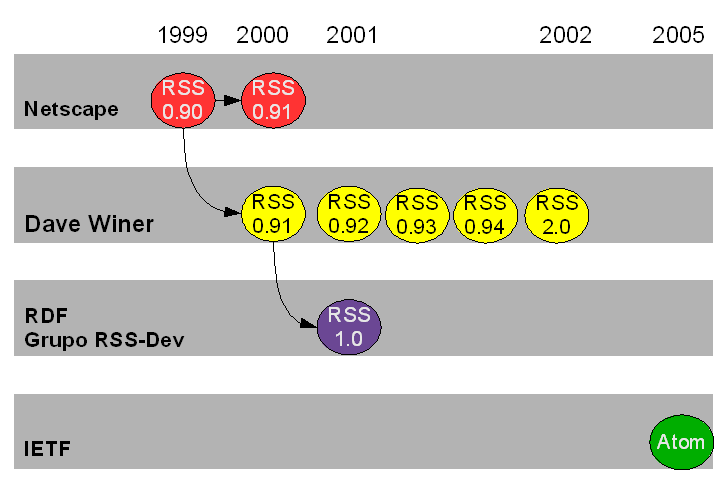
\includegraphics[width=10cm]{images/rssEvolution.png}
		\caption{Evolución de RSS}
		\label{fig:rssEvolution}
	\end{figure}

  \item \textbf{FOAF:} FOAF\footnote{\url{http://www.foaf-project.org/}}, acrónimo de 
	\emph{Friend-of-a-Friend}, se trata de un vocabulario RDF para describir 
	semánticamente información personal muy extendido (en 2004 se estimaba\cite{Li2005} 
	que existían alrededor de 1,2 millones de documentos FOAF) dentro del ámbito 
	de la web semántica.

\begin{figure} [H]
\lstset{language=RDF}
\begin{lstlisting}
<rdf:RDF
	xmlns:rdf="http://www.w3.org/1999/02/22-rdf-syntax-ns#"
	xmlns:rdfs="http://www.w3.org/2000/01/rdf-schema#"
	xmlns:foaf="http://xmlns.com/foaf/0.1/"
>

  <foaf:Person rdf:about="http://www.wikier.org/foaf.rdf#wikier">
    <foaf:name>Sergio Fdez</foaf:name>
    <foaf:title>Mr</foaf:title>
    <foaf:firstName>Sergio</foaf:firstName>
    <foaf:surname>Fdez</foaf:surname>
    <foaf:gender>Male</foaf:gender>
    <foaf:mbox>sergio@wikier.org</foaf:mbox>
  </foaf:Person>

</rdf:RDF>
\end{lstlisting}
\caption{Ejemplo de FOAF}
\label{fig:ejemplo.foaf}
\end{figure}

	Pudiendo describir relaciones (amigos, compañeros de trabajo, etc), intereses,
	proyectos y demás recursos de uso personal, de forma que se forme un grafo 
	uniendo todos ellos. El patrón\ref{fig:patternFOAF} siempre se repite.

	\begin{figure}[H]
		\centering
		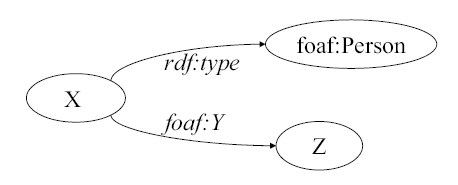
\includegraphics[width=7cm]{images/patron-foaf.png}
		\caption{Patrón de documentos FOAF}
		\label{fig:patternFOAF}
	\end{figure}

  \item \textbf{DOAP:} \emph{Description-of-a-Project\footnote{\url{http://usefulinc.com/doap}}} 
	es una idea similar a FOAF pero para describir todo tipo de proyectos.

\begin{figure}[H]
\lstset{language=RDF}
\begin{lstlisting}
<rdf:RDF xmlns:rdf="http://www.w3.org/1999/02/22-rdf-syntax-ns#" 
         xmlns:rdfs="http://www.w3.org/2000/01/rdf-schema#" 
         xmlns:doap="http://usefulinc.com/ns/doap#" 
         xmlns:foaf="http://xmlns.com/foaf/0.1/" 
         xmlns:admin="http://webns.net/mvcb/" 
>

  <doap:Project rdf:about="http://swaml.berlios.de/">

    <doap:name>Semantic Web Archive of Mailing Lists</doap:name>
    <doap:shortname>SWAML</doap:shortname>

    <doap:description>
      SWAML is a research project around the semantic web tecnologies 
      to publish the mailing lists archive into a RDF format.
    </doap:description>

    <doap:homepage rdf:resource="http://swaml.berlios.de/" />
    <doap:wiki rdf:resource="http://swaml.berlios.de/wiki" />
    <doap:license rdf:resource="http://usefulinc.com/doap/licenses/gpl" />

  </doap:Project>

</rdf:RDF>
\end{lstlisting}
\caption{Fichero DOAP de SWAML}
\label{fig:ejemplo.doap}
\end{figure}

  \item \textbf{EARL:} EARL\cite{EARL} (\emph{Evaluation and Report Language}, 
	en español \emph{Lenguaje de Evaluación de informes} es un vocabulario 
     	RDF para la grabación, transferencia y procesamiento de datos sobre 
	evaluaciones automáticas. Es usado por ejemplo por algunas herramientas
	de validación automática de la accesibilidad Web, como el
	TAW\footnote{\url{http://www.tawdis.net/}}, para expresar el
	resultado de sus evaluaciones.

\end{itemize}

\subsubsection{Otras aplicaciones de RDF}

\begin{itemize}
  \item \textbf{Framework Mozilla:} Firefox utiliza RDF internamente para 
	describir muchos aspectos del navegador. Por ejemplo un fichero como 
	el mostrado en la figura~\ref{fig:rdf.firefox} se utiliza en sus
	extensiones para describirlas semánticamente.

\begin{figure}[H]
\lstset{language=RDF}
\begin{lstlisting}
<?xml version="1.0" encoding="utf-8"?>

<rdf:RDF 
	xmlns:rdf="http://www.w3.org/1999/02/22-rdf-syntax-ns#"
	xmlns:em="http://www.mozilla.org/2004/em-rdf#"
>

  <rdf:Description rdf:about="urn:mozilla:install-manifest">
    <em:creator>Sergio Fdez</em:creator>
    <em:description>
      FOAFox, discover FOAF profiles in Firefox
    </em:description>
    <em:homepageURL>
      http://www.wikier.org/archivos/firefox/foafox/
    </em:homepageURL>
    <em:id>{5be0dd31-4194-4543-b29c-72248db06b71}</em:id>
    <em:name>FOAFox</em:name>
    <em:iconURL>chrome://foafox/skin/foafox.png</em:iconURL>
    <em:updateURL>
      http://www.wikier.org/archivos/mozilla/foafox/update.rdf
    </em:updateURL>
    <em:version>0.2.1</em:version>
    <em:targetApplication>
      <rdf:Description>
        <em:id>{ec8030f7-c20a-464f-9b0e-13a3a9e97384}</em:id>
        <em:minVersion>1.5</em:minVersion>
        <em:maxVersion>2.0.0.*</em:maxVersion>
      </rdf:Description>
    </em:targetApplication>
  </rdf:Description>

</rdf:RDF>
\end{lstlisting}
\caption{Ejemplo fichero RDF para describir una extensión de Mozilla Firefox}
\label{fig:rdf.firefox}
\end{figure}

\end{itemize}


\subsection{Futuro}

Hacia donde irá la Web Semántica es algo que sólo se sabrá con el tiempo, y quizás
en un plazo no más allá de 5 o 10 años. Por ahora es muy pronto para aventurar nada,
aunque si bien es cierto que el estado de adopción de la Web Semántica, en palabras
del propio Ivan Herman\footnote{\url{http://www.w3.org/2006/Talks/1109-Athens-IH/}}
(líder de la actividad de web semántica del W3C), crece a un ritmo imparable.

Históricamente han existido áreas de investigación vendidas en exceso como la 
panacea de la solución de todos los problemas de la humanidad; generando unas 
expectativas falsas que han hecho mucho daño a la comunidad científica.

Lo que si sabemos es que la Web Semántica será una Web mucho más \emph{útil}.
